\documentclass[12pt]{article}
 \usepackage[margin=1in]{geometry} 
\usepackage{amsmath,amsthm,amssymb,outlines}
\usepackage{graphicx,tikzsymbols,tcolorbox}
\renewcommand\qedsymbol{$\blacksquare$}
\tcbuselibrary{most}

% Defining new environments

\newtcolorbox{newtitle}{
  enhanced,
  colframe=black,
  colback=white,
  boxsep=5pt,
  arc=8pt,
  sharp corners=south,
  borderline={0.5pt}{0pt}{black},
  borderline={1.8pt}{-5pt}{black},
  after skip=30pt
}

\newtcolorbox[auto counter, number within=section]{theorem}[2][title]{
  enhanced,
title={Theorem \thetcbcounter \if\relax\detokenize{#2}\relax\else\ (#2)\fi},
  colframe=black,
  colback=white,
  colbacktitle=white,
  fonttitle=\bfseries,
  coltitle=black,
  attach boxed title to top left={yshift=-0.25mm-\tcboxedtitleheight/2,yshifttext=2mm-\tcboxedtitleheight/2, xshift=2mm},
  boxed title style={boxrule=0.5mm}
}

\newtcolorbox[auto counter, number within=section]{definition}{
  enhanced,
  title={Definition \thetcbcounter},
  colframe=black,
  colback=white,
  colbacktitle=white,
  fonttitle=\bfseries,
  coltitle=black,
  attach boxed title to top left={yshift=-0.25mm-\tcboxedtitleheight/2,yshifttext=2mm-\tcboxedtitleheight/2, xshift=2mm},
  boxed title style={boxrule=0.5mm}
}

\newtcolorbox[auto counter, number within=section]{fact}{
  enhanced,
  title={Fact \thetcbcounter},
  colframe=black,
  colback=white,
  colbacktitle=white,
  fonttitle=\bfseries,
  coltitle=black,
  attach boxed title to top left={yshift=-0.25mm-\tcboxedtitleheight/2,yshifttext=2mm-\tcboxedtitleheight/2, xshift=2mm},
  boxed title style={boxrule=0.5mm}
}

\newtcolorbox{newproof}{
  enhanced,
  frame hidden,
  colback=white,
  title={Proof.},
  fonttitle=\bfseries,
  coltitle=black,
  colbacktitle=white,
  boxed title style={boxrule=0.5mm},
  attach boxed title to top left={yshift=-0.25mm-\tcboxedtitleheight/2,yshifttext=2mm-\tcboxedtitleheight/2, xshift=2mm},
  borderline west={1.5pt}{8pt}{black},
  after upper={\hfill $\blacksquare$},
  after skip=30pt
}

\newtcolorbox[auto counter, number within=section]{uq}{
  enhanced,
  title=Question,
  colframe=red,
  colback=white,
  colbacktitle=white,
  fonttitle=\bfseries,
  coltitle=black,
  attach boxed title to top left={yshift=-0.25mm-\tcboxedtitleheight/2,yshifttext=2mm-\tcboxedtitleheight/2, xshift=2mm},
  boxed title style={boxrule=0.5mm}
}

\newtcolorbox[auto counter, number within=section]{aq}{
  enhanced,
  title=Question,
  colframe=green!50!black,
  colback=white,
  colbacktitle=white,
  fonttitle=\bfseries,
  coltitle=black,
  attach boxed title to top left={yshift=-0.25mm-\tcboxedtitleheight/2,yshifttext=2mm-\tcboxedtitleheight/2, xshift=2mm},
  boxed title style={boxrule=0.5mm}
}

\newtcolorbox{answer}{
  enhanced,
  frame hidden,
  colback=white,
  colframe=green!50!black,
  title={Answer},
  fonttitle=\bfseries,
  coltitle=black,
  colbacktitle=white,
  boxed title style={boxrule=0.5mm},
  attach boxed title to top left={yshift=-0.25mm-\tcboxedtitleheight/2,yshifttext=2mm-\tcboxedtitleheight/2, xshift=2mm},
  borderline west={1.5pt}{8pt}{green!50!black}
}

\newtcolorbox{sectionbox}{
  colback=black!10,
  colframe=black, 
  fonttitle=\bfseries\Large, 
  arc=4mm, 
  width=\textwidth
}

% Redefine section as well

% Renew commands later

\begin{document}

\begin{newtitle}
  \begin{center}
    \textbf{\Huge Complex Analysis Notes}
  \end{center}
  \textbf{Dahlen Elstran} \hfill \textbf{\today} \\
  Dr. Jingzhi Tie \hfill Spring 2025
\end{newtitle}

\section*{Introduction}

Let us begin by noting that every complex number $z$ can be written as $z=x+iy$, where $x,y \in \mathbb{R}$.

\begin{definition}
  A function is \textbf{holomorphic} at the point $z \in \mathbb{C}$ if the limit 
  \begin{equation*}
    \lim_{h \to 0} \frac{f(z+h)-f(z)}{h}, \text{ where } h \in \mathbb{C}
  \end{equation*}
  exists.
\end{definition}

\begin{aq}
  So is this just being differentiable for complex numbers?
\end{aq}
\begin{answer}
  Essentially, however because complex numbers have a value (radius) and an angle, $h$ can approach 0 from 
  infinitely many angles. So holomorphicity is much stronger than differentiablity; In the real case, it 
  is differentiable going left and right. For a function to be holomorphic at a point, it must be differentiable 
  from infinitely many angles.
\end{answer}

\begin{fact}
  If $f$ is holomorphic in $\Omega$, then for appropriate closed paths in $\Omega$, 
  \begin{equation*}
    \int_{\gamma} f(z)dz=0.
  \end{equation*}
\end{fact}

\begin{fact}
  If $f$ is holomorphic, then $f$ is indefinitely differentiable.
\end{fact}

\begin{uq}
  Why indefinitely differentiable? Why not indefinitely holomorphic?
\end{uq}

\begin{fact}
  If $f$ and $g$ are holomorphic functions in $\Omega$ which are equal in an arbitrarily samll disc in 
  $\omega$, then $f=g$ everywhere in $\Omega$.
\end{fact}

\begin{definition}
  The \textbf{zeta function},
  \begin{equation*}
    \zeta (s)=\sum^{\infty}_{n=1} \frac{1}{n^s}
  \end{equation*}
  is holomorphic in the half-plane Re($s$) $> 1$.
\end{definition}

\begin{definition}
  The \textbf{theta function} is the following:
  \begin{equation*}
    \Theta (z \vert \tau) = \sum^{\infty}_{n=-\infty} e^{\pi i n^2 \tau}e^{2\pi i n z}
  \end{equation*}
\end{definition}

\section{Preliminaries to Complex Analysis}

\subsection{Complex Numbers and the Complex Plane}

We can imagine complex numbers as an ordered pair of the two real numbers:
  
\par \begin{center} 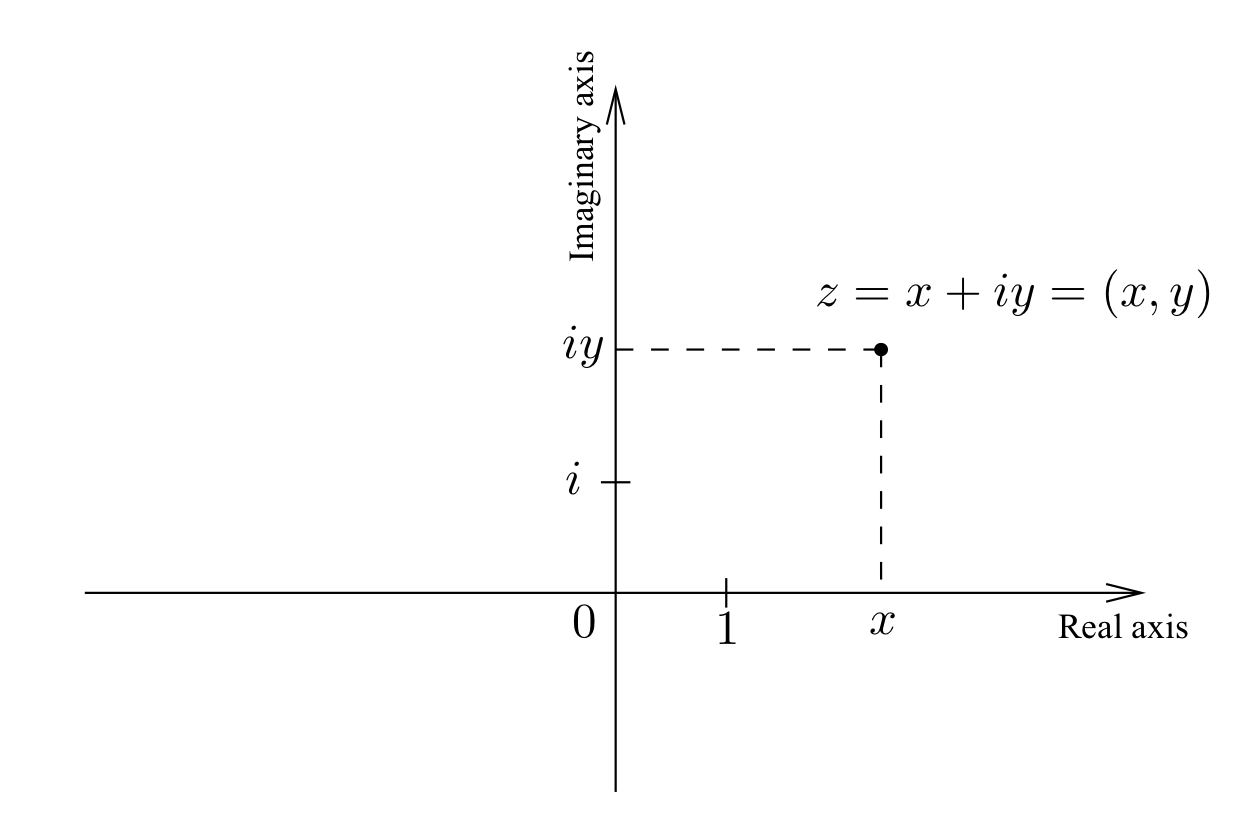
\includegraphics[scale=.2]{1-1.png} \end{center}

Addition and mulitplication are defined like so:

\begin{align*}
  z_1+z_2 &= (x_1+x_2)+i(y_1+y_2) \\
  z_1 * z_2 &= (x_1x_2 - y_1y_2) + i (x_1y_2+y_1x_2)
\end{align*}

It is easy to prove that commutativity, associativity, and distributivity hold for complex numbers. 
We can think about addition like adding two vectors in $\mathbb{R}^2$, and mulitplication like 
a rotation and dilation.

\begin{definition}
  The length, or absolute value of a complex number, is defined as the following:
  \begin{equation*}
    \vert z \vert = (x^2 + y^2)^{1/2}
  \end{equation*}
\end{definition}

Note that this is the same as taking the norm, or length, of a vector in $\mathbb{R}^2$, or even 
finding the length of the hypotenuse that is created by the $x$ and $y$ values.

\par The triangle equality holds: 

\begin{theorem}{Triangle Inequality}
  \begin{equation*}
    \vert z + w \vert \leq \vert z \vert + \vert w \vert
  \end{equation*}
  for all $z,x \in \mathbb{C}$.
\end{theorem}

From the triangle inequality, there comes this helpful fact as well:

\begin{fact}
  \begin{equation*}
    \vert \vert z \vert - \vert w \vert \vert \leq \vert z - w \vert 
  \end{equation*}
\end{fact}

You can imagine a complex conjugate, $\bar{z} = x - iy$, as a reflection across the real (horizontal) axis.

\par The following are also useful facts easily deduced:

\begin{fact}
  \begin{equation*}
    \text{Re} (z) = \frac{z+\bar{z}}{2} \text{ and } \text{Im} (z) = \frac{z-\bar{z}}{2i}
  \end{equation*}
\end{fact}

\begin{fact}
  \begin{equation*}
  \vert z \vert = z \bar{z} \text{ and, when } z \neq 0 \text{, } \frac{1}{z} = {\bar{z}}{\vert z \vert ^2}
  \end{equation*}
\end{fact}

\begin{definition}
  A complex number $z$'s \textbf{polar form} is written as $z=re^{i \theta}$, where $r > 0$, and 
  $\theta$ is referred to as the \textbf{argument} of $z$.
\end{definition}

A mathematical fact useful in Complex Analysis is $e^{i \theta} = \cos{\theta} + i \sin{\theta}$.

From the two previous statements, we can see that $r=\vert z \vert$, the length of $z$, and $\theta$ is the angle. 

\par \begin{center} 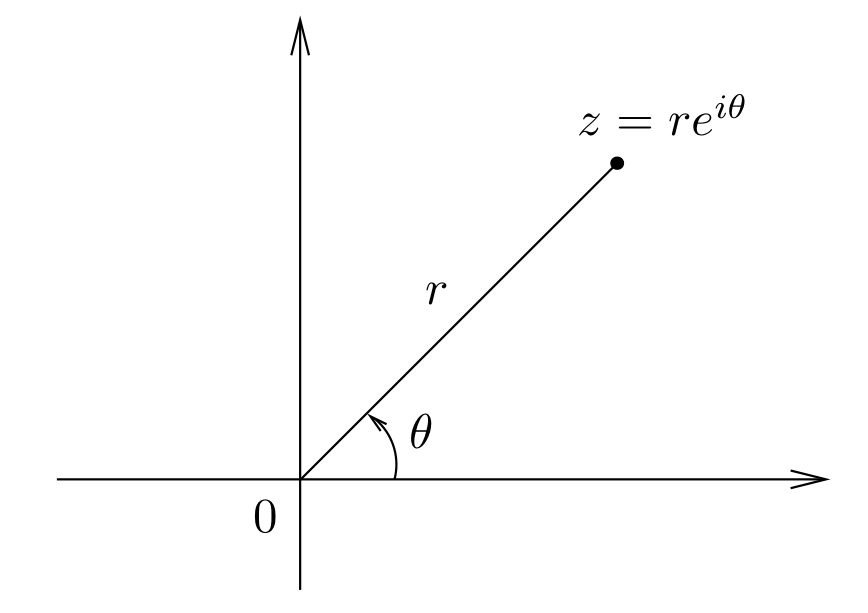
\includegraphics[scale=.2]{1-2.png} \end{center}

With this form, we can redefine mulitplication to be:

\begin{equation*}
  z = re^{i \theta}, w=se^{i \phi} \implies zw=rse^{i(\theta + \phi)}\
\end{equation*}

It is easier to see in this definition that mulitplication is simply a rotation ($\theta + \phi$), and 
a dilation ($rs$).

\begin{definition}
  A sequence $\{z_1, z_2, \dots \}$ of complex numbers is said to \textbf{converge} 
  to $w \in \mathbb{C}$ if 
  $$ \lim_{n \to \infty} \vert z_n - w \vert = 0 \text{ or,equivalently, } w = \lim_{n \to \infty} z_n. $$
\end{definition}


\end{document}
